\documentclass[11pt, a4paper]{article}

\usepackage[utf8]{inputenc}
\usepackage[T1]{fontenc}
\usepackage{amsmath, amssymb}
\usepackage{physics}
\usepackage{graphicx}
\usepackage{hyperref}
\usepackage{booktabs}
\usepackage{xcolor}
\usepackage{listings}
\usepackage{geometry}
\usepackage{float}

\geometry{margin=1in}
\hypersetup{colorlinks=true, linkcolor=blue!70!black, urlcolor=blue!60!black}

\graphicspath{{notebook_figures/}}

\lstset{
    language=Python,
    basicstyle=\ttfamily\small,
    keywordstyle=\color{blue!70!black}\bfseries,
    commentstyle=\color{green!50!black}\itshape,
    stringstyle=\color{red!60!black},
    numbers=left, numberstyle=\tiny\color{gray},
    breaklines=true, frame=single,
    backgroundcolor=\color{gray!5},
    showstringspaces=false
}

\title{OneBQF Notebook --- Walkthrough and Results}
\author{Notes on Chiotopoulos et al.\ (arXiv:2511.11458)}
\date{\today}

\begin{document}
\maketitle
\tableofcontents
\newpage

% ======================================================================
\section{Overview}

This document walks through the \texttt{example.ipynb} notebook from the
OneBQF repository, which demonstrates the 1-Bit Quantum Filter algorithm
for charged particle track reconstruction. The notebook sets up a
simulated particle detector, constructs a Hamiltonian encoding the
tracking problem as a linear system, solves it with a quantum algorithm,
and compares the result to the classical answer.

The paper behind this code is
\href{https://arxiv.org/abs/2511.11458}{``TrackHHL: A Quantum Computing
Algorithm for Track Reconstruction at the LHCb''} by Chiotopoulos et al.
The repository is at
\url{https://github.com/Xenofon-Chiotopoulos/OneBQF}.

% ======================================================================
\section{Problem Setup}

The goal is to reconstruct particle tracks in the LHCb VELO detector. In
the simulation, 64 particles originate from a single collision point
(Primary Vertex) and travel through 5 planar silicon detector layers. Each
particle leaves one hit per layer, giving 320 hits total.

The tracking problem is: given only the hits, figure out which ones belong
to the same particle. The approach is to enumerate all possible line
segments (``doublets'') connecting hits in adjacent layers, then determine
which segments are real (part of a track) and which are fake.

With 64 particles and 5 layers, there are $64 \times 64 = 4{,}096$
candidate segments per layer gap, times 4 gaps, giving $16{,}384$ total
candidate segments. Out of these, only $64 \times 4 = 256$ are real.

\subsection{Detector Configuration}

The notebook configures the detector as follows:

\begin{lstlisting}[caption={Detector and event setup}]
dz = 20                 # layer spacing: 20 mm
n_particles = [64]      # 64 particles in one collision event
layers = 5              # 5 detector layers
lx = [33, 33, 33, 33, 33]  # each layer is 33 mm wide
ly = [33, 33, 33, 33, 33]  # each layer is 33 mm tall
zs = [20, 40, 60, 80, 100] # z-positions in mm
\end{lstlisting}

The detector is idealised: measurement error is set to zero, there is no
multiple scattering, and no hits are dropped or added as ghosts. This
keeps the focus on testing the quantum algorithm rather than studying
detector effects.

% ======================================================================
\section{Event Display}

Figure~\ref{fig:event} shows the simulated event. The 5 vertical black
lines are the detector layers. Each line segment connects a hit in one
layer to a hit in the next. Green segments are the true (active) ones that
belong to real particle tracks. Gray/black segments are fake combinations
that do not correspond to any particle.

\begin{figure}[H]
\centering
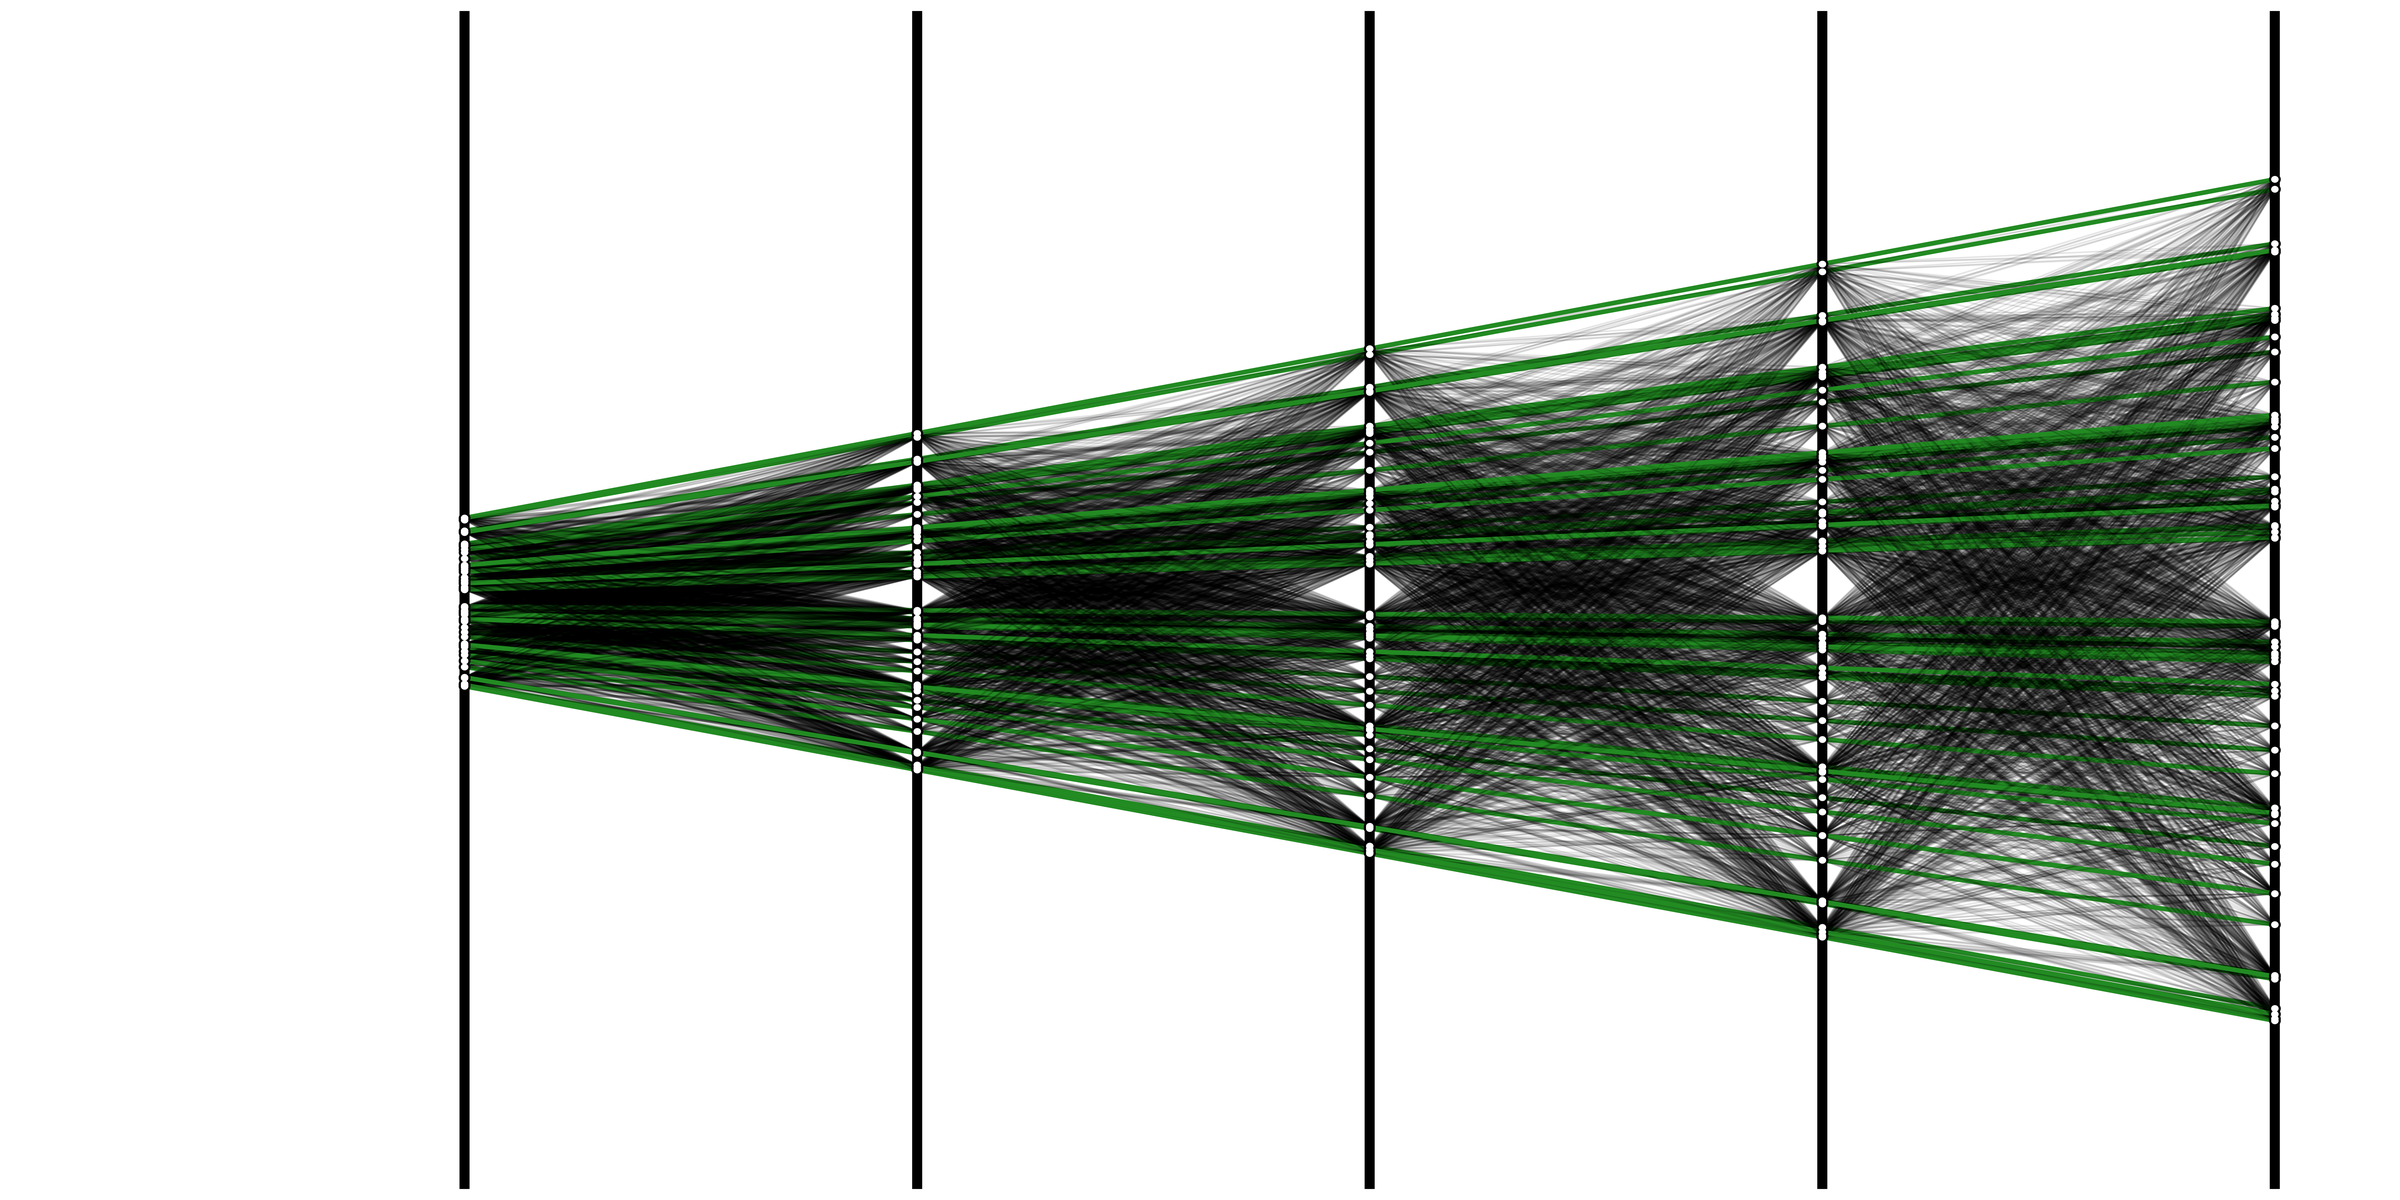
\includegraphics[width=\textwidth]{event_display.png}
\caption{2D event display for 64 particles traversing 5 detector layers.
Green lines are true track segments; gray lines are combinatorial fakes.
There are 16,384 candidate segments total, of which 256 are real.}
\label{fig:event}
\end{figure}

The figure illustrates the scale of the combinatorial problem. Most of the
line segments are wrong, and the true tracks are buried in a dense web of
fakes. The Hamiltonian approach assigns an energy to each configuration of
active/inactive segments, and the minimum-energy configuration is the one
where only the true track segments are turned on.

% ======================================================================
\section{The Hamiltonian and Linear System}

The tracking problem is encoded as a Hamiltonian with three terms:
\begin{equation}
    H(\vec{S}) = H_{\text{ang}}(\vec{S}, \epsilon) + \alpha\, H_{\text{spec}}(\vec{S}) + \beta\, H_{\text{gap}}(\vec{S})
\end{equation}

\begin{itemize}
    \item $H_{\text{ang}}$: rewards pairs of consecutive segments that are
          nearly collinear (angle $< \epsilon$). This is what identifies
          real tracks.
    \item $H_{\text{spec}}$: penalises segments for being active
          ($\alpha = 2.0$).
    \item $H_{\text{gap}}$: penalises segments for being inactive
          ($\beta = 1.0$).
\end{itemize}

The competition between these terms means that only segments forming
straight lines through multiple layers gain enough reward from
$H_{\text{ang}}$ to overcome the penalty from $H_{\text{spec}}$.

\subsection{From Hamiltonian to Linear System}

Each candidate segment $i$ is assigned a continuous variable $S_i$
representing how ``active'' it is. The full Hamiltonian is a quadratic
function of the segment state vector $\vec{S} = (S_1, S_2, \ldots,
S_N)^T$:
\begin{equation}
    H(\vec{S}) = \frac{1}{2}\,\vec{S}^{\,T} A\, \vec{S} \;-\; \vec{b}^{\,T}\vec{S}
\end{equation}

The matrix $A$ encodes all the physics. Its entries are:
\begin{itemize}
    \item \textbf{Diagonal:} $A_{ii} = \alpha + \beta$ for every segment.
          The two penalties work together: $\alpha$ (the spectral term)
          penalises a segment for being active, and $\beta$ (the gap term)
          penalises it for being inactive. Every segment starts with this
          baseline cost of $\alpha + \beta$ on the diagonal regardless of
          whether it is real or fake. In the notebook $\alpha = 2$ and
          $\beta = 1$, so every diagonal entry is $3.0$. Think of it as the
          ``default resistance'' each segment has against being turned on---the
          system needs a reason (aligned neighbours) to overcome it.
    \item \textbf{Off-diagonal:} $A_{ij} = -1$ if segments $i$ and $j$
          share a middle hit \emph{and} are nearly collinear (angle $<
          \epsilon$). Otherwise $A_{ij} = 0$. These $-1$ entries are the
          angular reward from $H_{\text{ang}}$: they lower the energy when
          both connected segments are active together. Since the matrix is
          symmetric ($A_{ij} = A_{ji}$), each connection appears twice.
\end{itemize}

The vector $\vec{b}$ has every entry equal to $\beta$. Since $\beta = 1$
here, $\vec{b} = (1, 1, \ldots, 1)^T$.

To find the configuration that minimises the energy, we take the gradient
and set it to zero:
\begin{equation}
    \nabla_{\vec{S}}\, H = A\,\vec{S} - \vec{b} = 0
    \quad\Longrightarrow\quad
    A\,\vec{S} = \vec{b}
\end{equation}

This is an ordinary linear system. The solution vector $\vec{S}$ gives a
continuous ``pseudo-state'' for each segment: segments with high $S_i$ are
likely part of a real track, and segments with low $S_i$ are likely fakes.

To see why this works intuitively, think about solving $A\vec{S} =
\vec{b}$ one row at a time. Row $i$ says:
\begin{equation}
    (\alpha + \beta)\,S_i \;+\; \sum_{j\,:\, A_{ij}=-1} (-1)\cdot S_j \;=\; \beta
\end{equation}
If segment $i$ belongs to a real track, it has aligned neighbours with
$A_{ij} = -1$. Those neighbours are also active (high $S_j$), so the
negative sum subtracts from the left side, and $S_i$ must be \emph{larger}
to satisfy the equation. A fake segment has no aligned neighbours
(all off-diagonal entries in its row are zero), so it only sees the full
$(\alpha + \beta)$ on the diagonal and ends up with a small value:
$S_i = \beta / (\alpha + \beta) = 1/3 \approx 0.33$. That is exactly the
baseline you see in the classical solution plot for inactive segments.

The notebook constructs this with:

\begin{lstlisting}[caption={Hamiltonian construction}]
ham = SimpleHamiltonian(epsilon=1e-7, alpha=2.0, beta=1.0)
ham.construct_hamiltonian(event=event_tracks, convolution=False)
\end{lstlisting}

For the full 64-particle, 5-layer event this produces a $16{,}384 \times
16{,}384$ sparse matrix $A$ and a right-hand-side vector $\vec{b}$ of
length $16{,}384$.

Figure~\ref{fig:heatmap} shows the matrix $A$ for a minimal example (2
particles, 3 layers, giving $2^2 \times 2 = 8$ candidate segments). Three
types of entries are visible:
\begin{itemize}
    \item \textbf{Dark red ($+3.0$, diagonal):} The $(\alpha + \beta)$
          baseline penalty on every segment, as described above.
    \item \textbf{Dark blue ($-1.0$):} There are exactly 4 of these in the
          matrix, forming 2 symmetric pairs. Each pair is one true track
          connection---two consecutive segments from the same particle that
          share a middle hit and point in the same direction. With 2
          particles and 2 layer gaps there are exactly 2 such connections
          (one per track), and each appears twice because $A_{ij} = A_{ji}$.
          These are the \emph{only} real segment links in the entire matrix.
    \item \textbf{Light blue ($0$, most of the matrix):} All remaining
          entries. These segment pairs have no coupling---either they do
          not share a middle hit at all, or they share a hit but bend too
          sharply (angle $> \epsilon$) to be from the same track. This
          includes the 4 fake cross-particle segments that connect a hit
          from one particle to a hit from the other; those segments share
          middle hits but fail the angle test, so they get zero.
\end{itemize}

\begin{figure}[H]
\centering
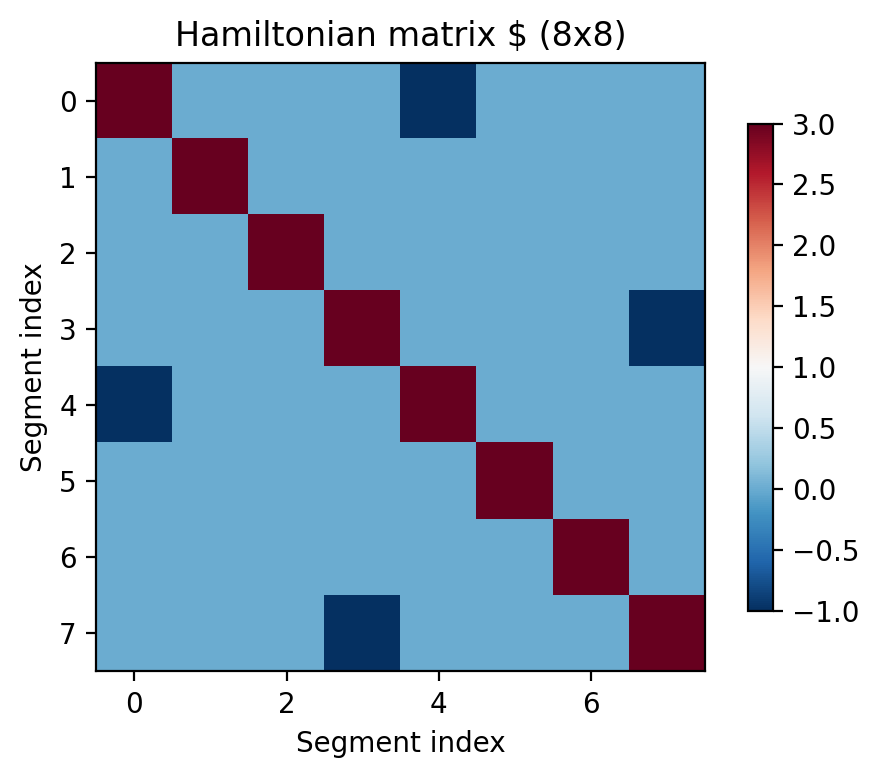
\includegraphics[width=0.55\textwidth]{hamiltonian_heatmap.png}
\caption{Hamiltonian matrix $A$ for a minimal example (2 particles, 3
layers, 8 segments). Dark red diagonal entries are $\alpha + \beta =
3.0$. Dark blue off-diagonal entries ($-1$) mark aligned, connected
segment pairs. Light blue entries are zero (no coupling).}
\label{fig:heatmap}
\end{figure}

For the full 64-particle case, the matrix has the same structure but is
$16{,}384 \times 16{,}384$ with 16,768 nonzero entries (extremely
sparse---$99.99\%$ zeros). The solver only needs to find the 256 segments
whose $S_i$ values are large---the rest are automatically suppressed by
the diagonal penalty.

% ======================================================================
\section{The OneBQF Quantum Circuit}

We now have a linear system $A\vec{S} = \vec{b}$ that encodes the
tracking problem. On a classical computer we would just use conjugate
gradient or Gaussian elimination. On a quantum computer, we use a
quantum algorithm called HHL (Harrow-Hassidim-Lloyd) that can in
principle solve linear systems exponentially faster.

The catch is that HHL in its full form requires many qubits and very deep
circuits. The 1-Bit Quantum Filter (OneBQF) is a drastically simplified
version that trades precision for practicality. Before explaining how it
works, we need a few quantum computing basics.

\subsection{Quick Quantum Background}

A \textbf{qubit} is the quantum analogue of a classical bit. A classical
bit is either 0 or 1. A qubit can be in a \textbf{superposition} of both:
$\ket{\psi} = \alpha\ket{0} + \beta\ket{1}$, where $\alpha$ and $\beta$
are complex numbers satisfying $|\alpha|^2 + |\beta|^2 = 1$. When you
\textbf{measure} the qubit, you get 0 with probability $|\alpha|^2$ and 1
with probability $|\beta|^2$---the superposition collapses.

With $n$ qubits you can represent a superposition over $2^n$ states
simultaneously. This is how quantum computers encode exponentially large
vectors using only a few qubits: 5 qubits can hold a superposition over
$2^5 = 32$ basis states, where each state has its own amplitude.

A \textbf{quantum gate} is an operation that transforms qubit states. Some
key gates used in this circuit:
\begin{itemize}
    \item \textbf{H (Hadamard)}: puts a qubit into an equal superposition
          of $\ket{0}$ and $\ket{1}$. Applied to $n$ qubits, it creates a
          uniform superposition over all $2^n$ states.
    \item \textbf{X (NOT)}: flips $\ket{0} \leftrightarrow \ket{1}$, like
          a classical NOT gate.
    \item \textbf{CNOT}: a two-qubit gate that flips the target qubit only
          if the control qubit is $\ket{1}$.
    \item \textbf{$R_x(\theta)$}: rotates a qubit by angle $\theta$ around
          the x-axis of the Bloch sphere (a smooth, partial rotation).
    \item \textbf{P($\phi$)}: adds a phase $\phi$ to the $\ket{1}$
          component of a qubit.
    \item \textbf{Controlled gates}: any gate can be made
          ``controlled''---it only acts on its target qubit(s) when one or
          more control qubits are in state $\ket{1}$. In the circuit
          diagram, control qubits are shown as dots connected by vertical
          lines to the gate they control.
\end{itemize}

\subsection{The Three Registers}

The circuit uses three groups of qubits, called \textbf{registers}, each
with a different job:

\begin{enumerate}
    \item \textbf{Time register} (1 qubit, labelled ``time'' in the
          circuit): This qubit performs \emph{phase estimation}---it
          figures out information about the eigenvalues of the matrix $A$.
          In full HHL you would use many time qubits to get precise
          eigenvalue estimates. The ``1-Bit'' in OneBQF means we use just
          one, giving only a single bit of precision: enough to distinguish
          ``eigenvalue corresponds to an active segment'' from ``eigenvalue
          corresponds to an inactive segment.'' This is the key
          simplification that makes the circuit small.

    \item \textbf{System register} ($\log_2 N$ qubits, labelled $b_0,
          b_1, b_2, \ldots$): These qubits encode the problem. At the
          start, they hold the input vector $\vec{b}$. At the end (after
          post-selection), they hold the solution $\vec{S}$. With $n$
          system qubits, you can represent a vector of length $2^n$ as
          amplitudes in superposition. For the 64-particle problem, the
          code pads the matrix to $32 \times 32$, so the system register
          uses $\log_2(32) = 5$ qubits.

    \item \textbf{Ancilla register} (1 qubit, labelled ``ancilla''): This
          is a helper qubit used for \emph{post-selection}. The circuit is
          designed so that this qubit ends up as $\ket{1}$ precisely when
          the system register contains the solution we want. After running
          the circuit many times, we \emph{throw away} all the runs where
          the ancilla measured 0 and only keep the runs where it measured
          1. This filtering step is what extracts the answer.
\end{enumerate}

For the 64-particle, 5-layer problem: $1 + 5 + 1 = 7$ qubits total.
That is remarkably few qubits for a problem with 16,384 segments---it
works because the segments are encoded as amplitudes in superposition,
not as individual qubits.

\begin{lstlisting}[caption={Building and running the quantum circuit}]
hhl_solver = onebqf(matrix_A, vector_b,
    num_time_qubits=1,   # 1-bit phase estimation
    shots=10000,          # number of measurement repetitions
    debug=False)

circuit = hhl_solver.build_circuit()
counts = hhl_solver.run(use_noise_model=False, backend_name=None)
quantum_solution, total_success = hhl_solver.get_solution()
\end{lstlisting}

\subsection{Circuit Structure}

Figure~\ref{fig:circuit} shows the circuit for a small example (2
particles, 3 layers, 5 qubits). Reading left to right, the circuit has
five stages:

\begin{enumerate}
    \item \textbf{State preparation (the H gates on the left):}
          Hadamard gates are applied to every system qubit ($b_0, b_1,
          b_2$). This puts the system register into a uniform
          superposition: every basis state has the same amplitude. That
          uniform superposition is the quantum encoding of our input vector
          $\vec{b} = (1, 1, \ldots, 1)^T$ (after normalisation). A
          Hadamard is also applied to the time qubit, putting it into
          superposition so it can ``probe'' both eigenvalue classes at once.

    \item \textbf{1-Bit Quantum Phase Estimation (QPE):}
          This is the core of the algorithm. The goal is to write
          information about the eigenvalues of $A$ into the time qubit.

          The matrix $A$ has eigenvalues (special numbers that characterise
          it). The key insight is that eigenvalues associated with
          \emph{active} segments are different from those associated with
          \emph{inactive} segments. QPE uses a controlled version of the
          time-evolution operator $e^{iAt}$ to ``kick'' the phase of the
          time qubit by an amount proportional to each eigenvalue.

          In the circuit diagram, this is implemented by the
          controlled-$R_x$ gates (the red/blue boxes on $b_2$ controlled
          by the time qubit) surrounded by X gates on $b_0$ and $b_1$.
          These implement the \textbf{Suzuki-Trotter decomposition}: instead
          of computing the exact matrix exponential $e^{iAt}$ (which would
          be very expensive), we approximate it as a product of simple
          rotations, one for each interacting pair of segments in the
          Hamiltonian. The X gates around each rotation select which
          specific basis states the rotation acts on---they ``address'' the
          right segment pairs from the matrix.

          After the controlled rotations, an inverse QFT (Quantum Fourier
          Transform, labelled IQFT) converts the accumulated phase into a
          measurable bit on the time qubit. With 1 time qubit, the result
          is binary: the time qubit ends up as $\ket{0}$ for one class of
          eigenvalue and $\ket{1}$ for the other.

    \item \textbf{Ancilla flip (the X-CNOT-X in the middle):}
          Now the time qubit holds a 1-bit label: $\ket{0}$ for active
          segments and $\ket{1}$ for inactive ones (or vice versa,
          depending on the eigenvalue structure). We want to flag the
          \emph{active} case. The X-CNOT-X gadget works as follows:
          \begin{itemize}
              \item X flips the time qubit ($\ket{0} \to \ket{1}$,
                    $\ket{1} \to \ket{0}$).
              \item CNOT copies the (now-flipped) time qubit into the
                    ancilla.
              \item X flips the time qubit back.
          \end{itemize}
          The net effect: the ancilla becomes $\ket{1}$ when the time qubit
          was $\ket{0}$ (the active-segment case). The ancilla is now our
          ``flag'' for a successful result.

    \item \textbf{Uncompute QPE (the right half):}
          The entire QPE circuit is run \emph{in reverse} (QFT instead of
          IQFT, rotations with negated angles). This ``uncomputes'' the
          phase estimation, returning the time qubit to a clean state. This
          step is necessary so that the time qubit does not remain entangled
          with the system register---if it stayed entangled, measuring the
          system qubits would give scrambled results. After uncomputation,
          all the useful information is in the system register and the
          ancilla.

    \item \textbf{Measurement (the meter symbols on the right):}
          All qubits are measured. Each measurement collapses the
          superposition and gives a definite bitstring (e.g.\
          ``\texttt{01101}'' for the system register, ``\texttt{1}'' for
          the ancilla). Since quantum measurement is probabilistic, we run
          the circuit many times (10,000 ``shots'' in the notebook) and
          collect statistics.
\end{enumerate}

\begin{figure}[H]
\centering
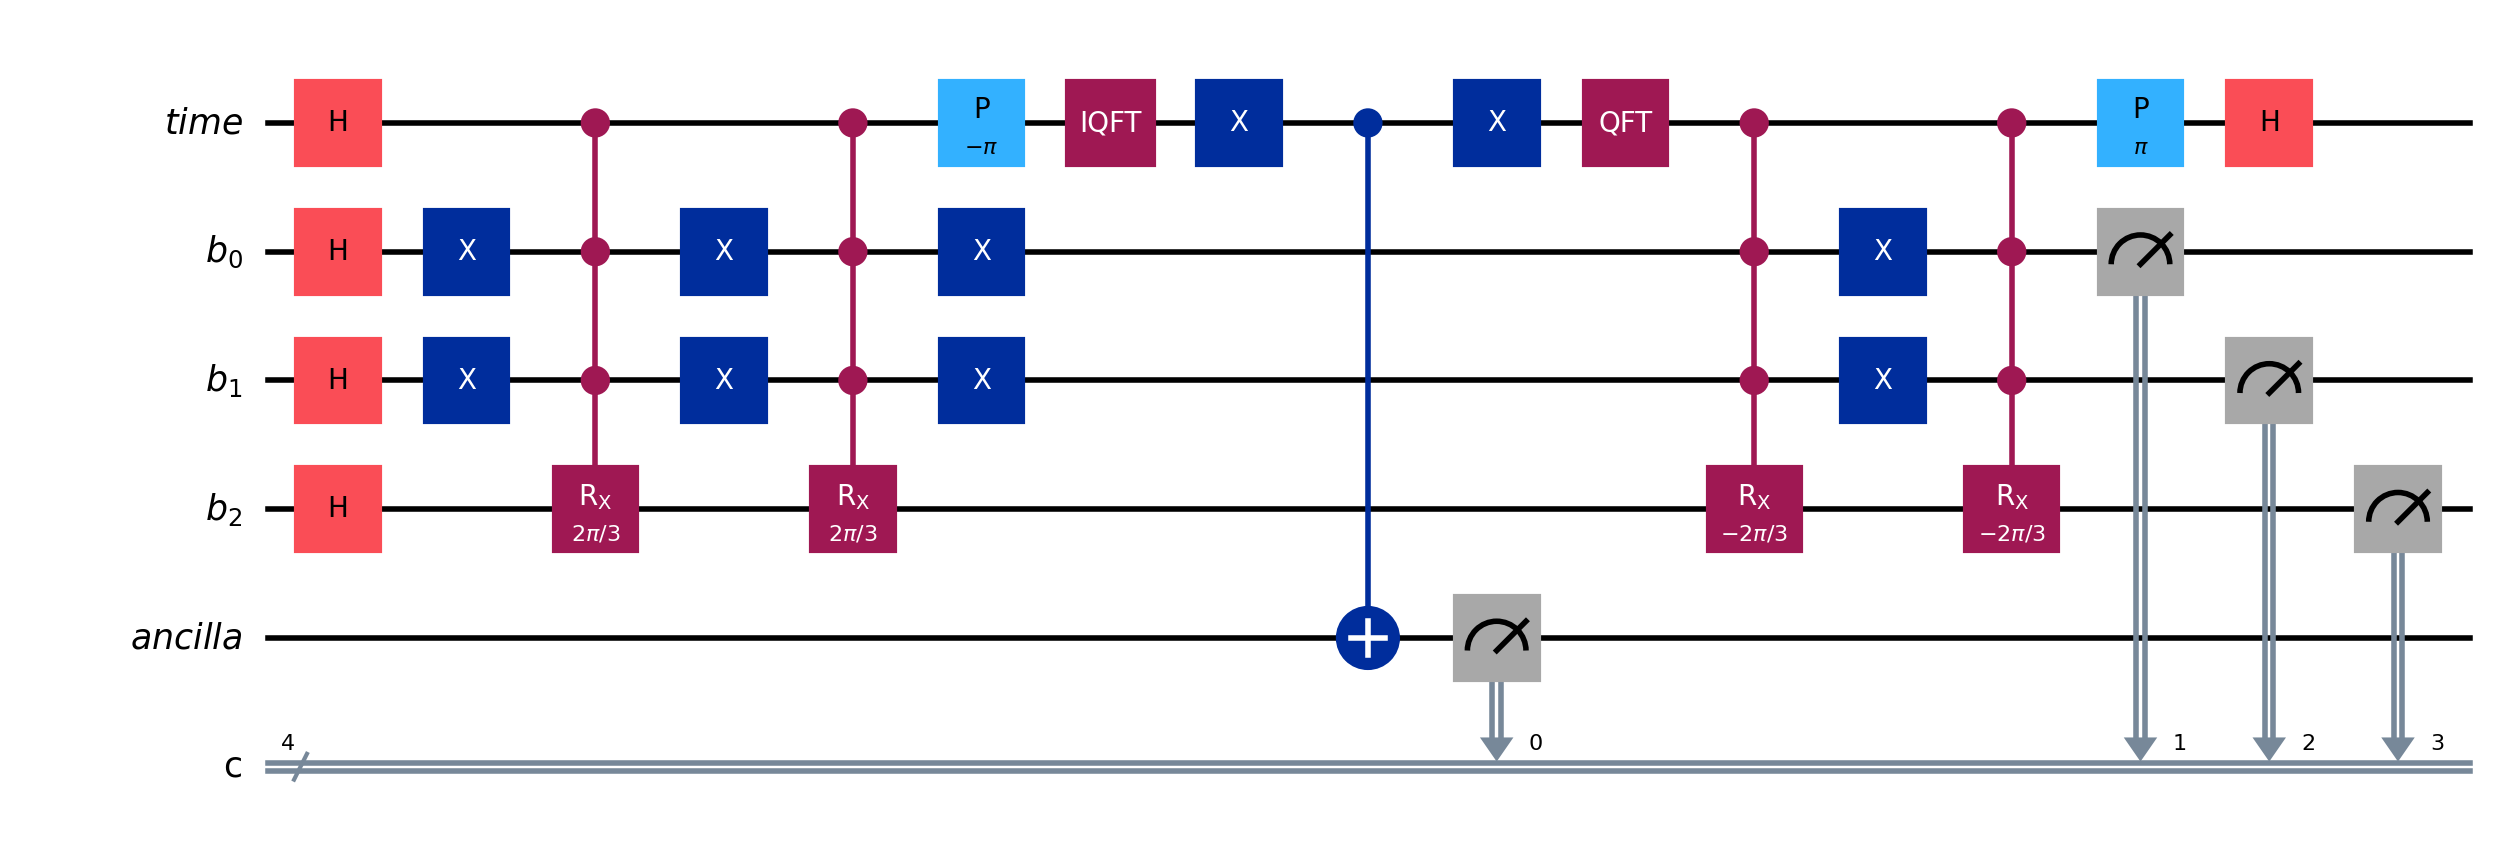
\includegraphics[width=\textwidth]{circuit_diagram.png}
\caption{OneBQF circuit for 2 particles and 3 layers (5 qubits total: 1
time, 3 system, 1 ancilla). Reading left to right: Hadamard gates prepare
the input, controlled-$R_x$ rotations with X gates implement
Suzuki-Trotter QPE, the X-CNOT-X gadget flags the ancilla, the reverse
QPE uncomputes, and meters measure everything.}
\label{fig:circuit}
\end{figure}

\subsection{Solution Extraction}

The circuit has been run 10,000 times. Each run gives a bitstring for the
system register and a single bit for the ancilla. The solution is
extracted in four steps:

\begin{enumerate}
    \item \textbf{Post-selection:} Throw away every shot where the ancilla
          measured $\ket{0}$. Only keep the shots where ancilla $=
          \ket{1}$---these are the ones where the circuit successfully
          flagged an active-segment component. Not every shot succeeds; the
          \emph{success probability} depends on the problem size (roughly
          $1/\sqrt{N}$, so a few percent for 64 particles).

    \item \textbf{Counting:} Among the kept shots, count how many times
          each system-register bitstring appeared. For example, if
          bitstring ``\texttt{00101}'' appeared 300 times out of 500
          successful shots, its probability is $p = 300/500 = 0.6$. Each
          bitstring corresponds to one segment index (``\texttt{00101}'' =
          index 5 in binary).

    \item \textbf{Square root:} Quantum measurement gives probabilities,
          but the solution $\vec{S}$ is encoded in \emph{amplitudes}. Since
          probability $=$ $|\text{amplitude}|^2$, we take the square root:
          $S_i = \sqrt{p_i}$. Segments that appeared frequently (high
          probability) get large $S_i$ values; segments that never appeared
          get $S_i = 0$.

    \item \textbf{Normalisation:} Divide the whole vector by its norm so
          that it has unit length. The quantum algorithm only gives the
          \emph{direction} of $\vec{S}$, not its absolute scale, since
          everything is normalised in quantum mechanics.
\end{enumerate}

The result is a vector where active segments have nonzero values and
inactive segments are exactly zero---no threshold needed. This clean
binary separation is a side-effect of the coarse Suzuki-Trotter
approximation ($n=1$, $t=1$): it does not faithfully reproduce all
eigenvalues of $A$, but it maps inactive-segment eigenvalues to exactly
the same phase, which the post-selection then kills completely.

% ======================================================================
\section{Classical Solution}

The classical solution is obtained by solving $A\vec{S} = \vec{b}$ using
the conjugate gradient method, then applying a threshold $T = 0.45$ to
convert the continuous solution into binary labels.

Figure~\ref{fig:classical} shows the result. The left panel is the raw
classical solution vector---each bar is one of the 16,384 segments. Bars
above the red dashed line ($T = 0.45$) are classified as active. The
active segments cluster at solution values of roughly 0.6--0.8, while the
inactive ones sit at around 0.1--0.33. There is a clear gap around the
threshold, making the classification unambiguous.

The right panel shows the discretised ground truth after thresholding:
256 out of 16,384 segments are active. These are exactly the
$64 \times 4 = 256$ true track segments.

\begin{figure}[H]
\centering
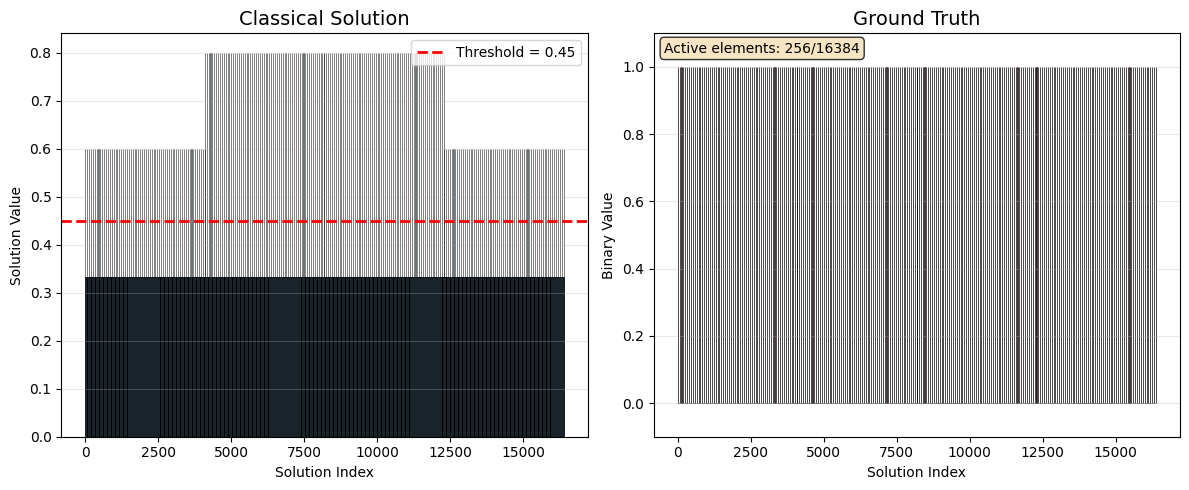
\includegraphics[width=\textwidth]{classical_solution.png}
\caption{Classical solution. Left: continuous solution values for all
16,384 segments with threshold $T = 0.45$ (red dashed line). Right:
binary ground truth after thresholding, showing 256 active segments out
of 16,384.}
\label{fig:classical}
\end{figure}

% ======================================================================
\section{Quantum Solution}

Figure~\ref{fig:quantum} shows the quantum solution from the 1-Bit
Quantum Filter. The shape of the solution is notably different from the
classical one: instead of a spread of values between 0 and 0.8, the
quantum solution has a handful of sharp spikes at $\sim$0.12 (active
segments) while everything else is completely suppressed to zero.

This is a direct consequence of the coarse Suzuki-Trotter approximation
($n = 1$, $t = 1$) used in the algorithm. While this approximation does
not faithfully reproduce the eigenvalues of $A$, it has the useful side
effect of pushing all inactive segment amplitudes to exactly zero. The
output is effectively binary without even needing to apply a threshold.

The right panel again shows 256 active elements out of 16,384, matching
the classical ground truth exactly.

\begin{figure}[H]
\centering
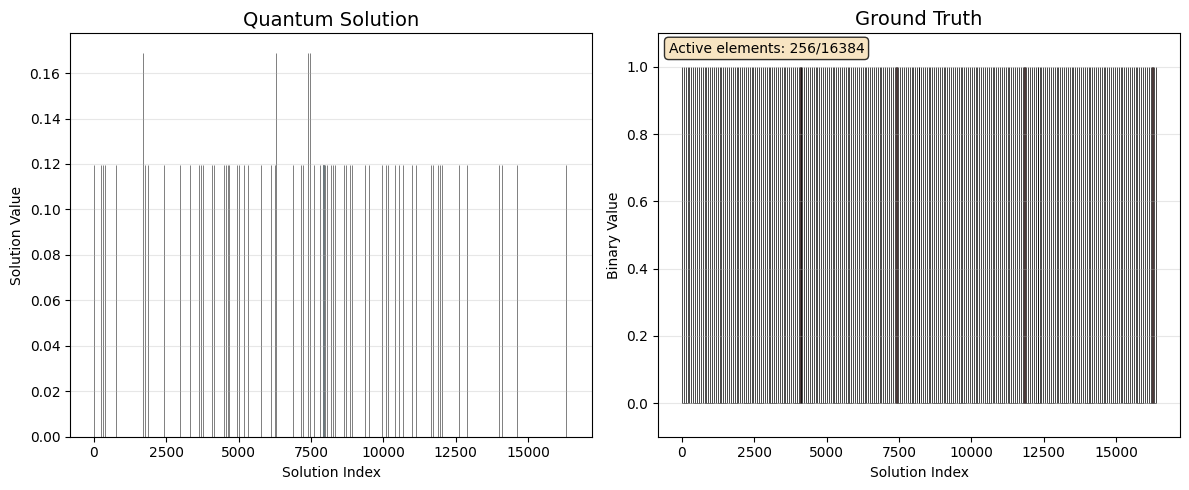
\includegraphics[width=\textwidth]{quantum_solution.png}
\caption{Quantum solution from the 1-Bit Quantum Filter. Left: solution
values showing sharp spikes at active segments and complete suppression
of inactive ones. Right: binary ground truth (256/16,384 active),
identical to the classical result.}
\label{fig:quantum}
\end{figure}

% ======================================================================
\section{Solution Comparison}

The notebook directly compares the two solutions:

\begin{lstlisting}[caption={Comparing quantum and classical active segments}]
classical_solution = ham.solve_classicaly()
T = .45
discretized_classical = (classical_solution > T).astype(int)

set1 = set(np.nonzero(discretized_classical)[0])
set2 = set(np.nonzero(quantum_solution)[0])
print("Solutions match", set1 - set2)
\end{lstlisting}

\begin{verbatim}
Solutions match set()
\end{verbatim}

The empty set means every segment that the classical solver identified as
active was also identified by the quantum solver. The 1-Bit Quantum
Filter reproduces the classical answer perfectly for this problem.

A visual comparison of the two solutions:

\begin{center}
\begin{tabular}{lcc}
\toprule
& \textbf{Classical} & \textbf{Quantum (OneBQF)} \\
\midrule
Active segments found  & 256 & 256 \\
Total segments         & 16,384 & 16,384 \\
Solution value (active)   & $\sim$0.6--0.8 & $\sim$0.12 \\
Solution value (inactive) & $\sim$0.1--0.33 & exactly 0 \\
Threshold needed?       & Yes ($T = 0.45$) & No (already binary) \\
Mismatch with truth     & 0 & 0 \\
\bottomrule
\end{tabular}
\end{center}

The key difference is in the shape of the solution. The classical solver
produces a smooth spectrum where active and inactive segments overlap
somewhat near the threshold. The quantum solver produces a clean binary
separation with no ambiguity, because the Trotter approximation naturally
suppresses all noise contributions.

% ======================================================================
\section{Circuit Statistics}

The notebook reports the gate counts and depth of the decomposed circuit:

\begin{lstlisting}[caption={Circuit statistics}]
circuit_depth = circuit.decompose().decompose()
    .decompose().decompose().decompose().depth()
circuit_statistics = circuit.decompose().decompose()
    .decompose().decompose().decompose().count_ops()
\end{lstlisting}

\begin{verbatim}
Circuit Depth: 507
Circuit Statistics: OrderedDict({
    'u': 365, 'cx': 321, 'u3': 144, 'measure': 6
})
\end{verbatim}

\begin{center}
\begin{tabular}{lr}
\toprule
\textbf{Metric} & \textbf{Value} \\
\midrule
Circuit depth (sequential gate chain) & 507 \\
CX (CNOT) gates (two-qubit)           & 321 \\
U gates (single-qubit rotations)       & 365 \\
U3 gates (single-qubit rotations)      & 144 \\
Measurements                           & 6 \\
Total qubits                           & 7 \\
\bottomrule
\end{tabular}
\end{center}

For a linear system of dimension 16,384, a circuit depth of 507 and only
321 two-qubit gates is remarkably small. The paper reports that the naive
HHL implementation for a much smaller problem (5 particles, 3 layers)
requires over 14 million gates. The 1-Bit approach reduces this by roughly
three orders of magnitude.

\subsection{TKET Optimisation}

The notebook also runs the circuit through TKET, Quantinuum's quantum
circuit compiler, which performs peephole optimisation (combining and
cancelling adjacent gates):

\begin{lstlisting}[caption={TKET optimisation}]
from pytket.extensions.qiskit import qiskit_to_tk
from pytket.passes import FullPeepholeOptimise

circuit_tk = qiskit_to_tk(decomposed_circuit)
FullPeepholeOptimise().apply(circuit_tk)
\end{lstlisting}

\begin{verbatim}
Gates: Counter({OpType.CX: 321, OpType.TK1: 310, OpType.Measure: 6})
Depth: 439
\end{verbatim}

TKET reduces the circuit depth from 507 to 439 (about 13\%). The CX gate
count stays at 321, indicating that the two-qubit gate structure was
already close to optimal. The single-qubit gates are merged from
$365 + 144 = 509$ into 310 TK1 gates.

% ======================================================================
\section{Complexity Comparison}

For reference, Table~\ref{tab:complexity} reproduces the paper's
comparison of different HHL implementations for 5 particles and 3 layers,
transpiled for IBM hardware. The 1-Bit approach achieves a roughly
$1{,}000\times$ reduction in total gate count.

\begin{table}[H]
\centering
\begin{tabular}{lrrr}
\toprule
\textbf{Method} & \textbf{Total Gates} & \textbf{2-Qubit Gates} & \textbf{Reduction} \\
\midrule
Naive HHL                & 14,515,229 & 7,107,317 & $1\times$ \\
Qiskit O3 transpilation  & 1,089,295  & 501,066   & $13\times$ \\
+ Suzuki-Trotter         & 257,367    & 120,171   & $56\times$ \\
+ 1-Bit Phase Estimation & 11,547     & 8,780     & $\sim 1{,}000\times$ \\
\bottomrule
\end{tabular}
\caption{Gate counts for 5 particles, 3 layers (14 qubits), transpiled
for IBM Hanoi (from the paper, Table 1).}
\label{tab:complexity}
\end{table}

The two sources of improvement are:
\begin{enumerate}
    \item \textbf{Suzuki-Trotter decomposition}: replaces the exact matrix
          exponential with a first-order product formula, cutting the gate
          count significantly.
    \item \textbf{1-Bit Phase Estimation}: reduces the QPE register from
          multiple qubits to a single qubit, which eliminates an entire
          layer of controlled operations. This also reduces the overall
          qubit count from $O(2\log_2 N + 2)$ to $O(\log_2 N + 3)$.
\end{enumerate}

% ======================================================================
% PART II --- SCALING AND NOISE ANALYSIS (from the paper's data)
% ======================================================================

\newpage
\section{Segment Efficiency Analysis}

The example notebook runs on an idealised detector with zero noise. A
separate analysis (from \texttt{plot\_segement\_analysis.ipynb}) studies
how well the Hamiltonian-based segment pairing performs as the number of
particles increases under more realistic conditions: a fixed angular
threshold of $\epsilon = 0.002$ (2~mrad), measurement resolution of
5~$\mu$m, and multiple scattering of 0.1~mrad. Each configuration is
repeated 100 times to gather statistics.

Figure~\ref{fig:segment} shows the results across four panels.

\begin{figure}[H]
\centering
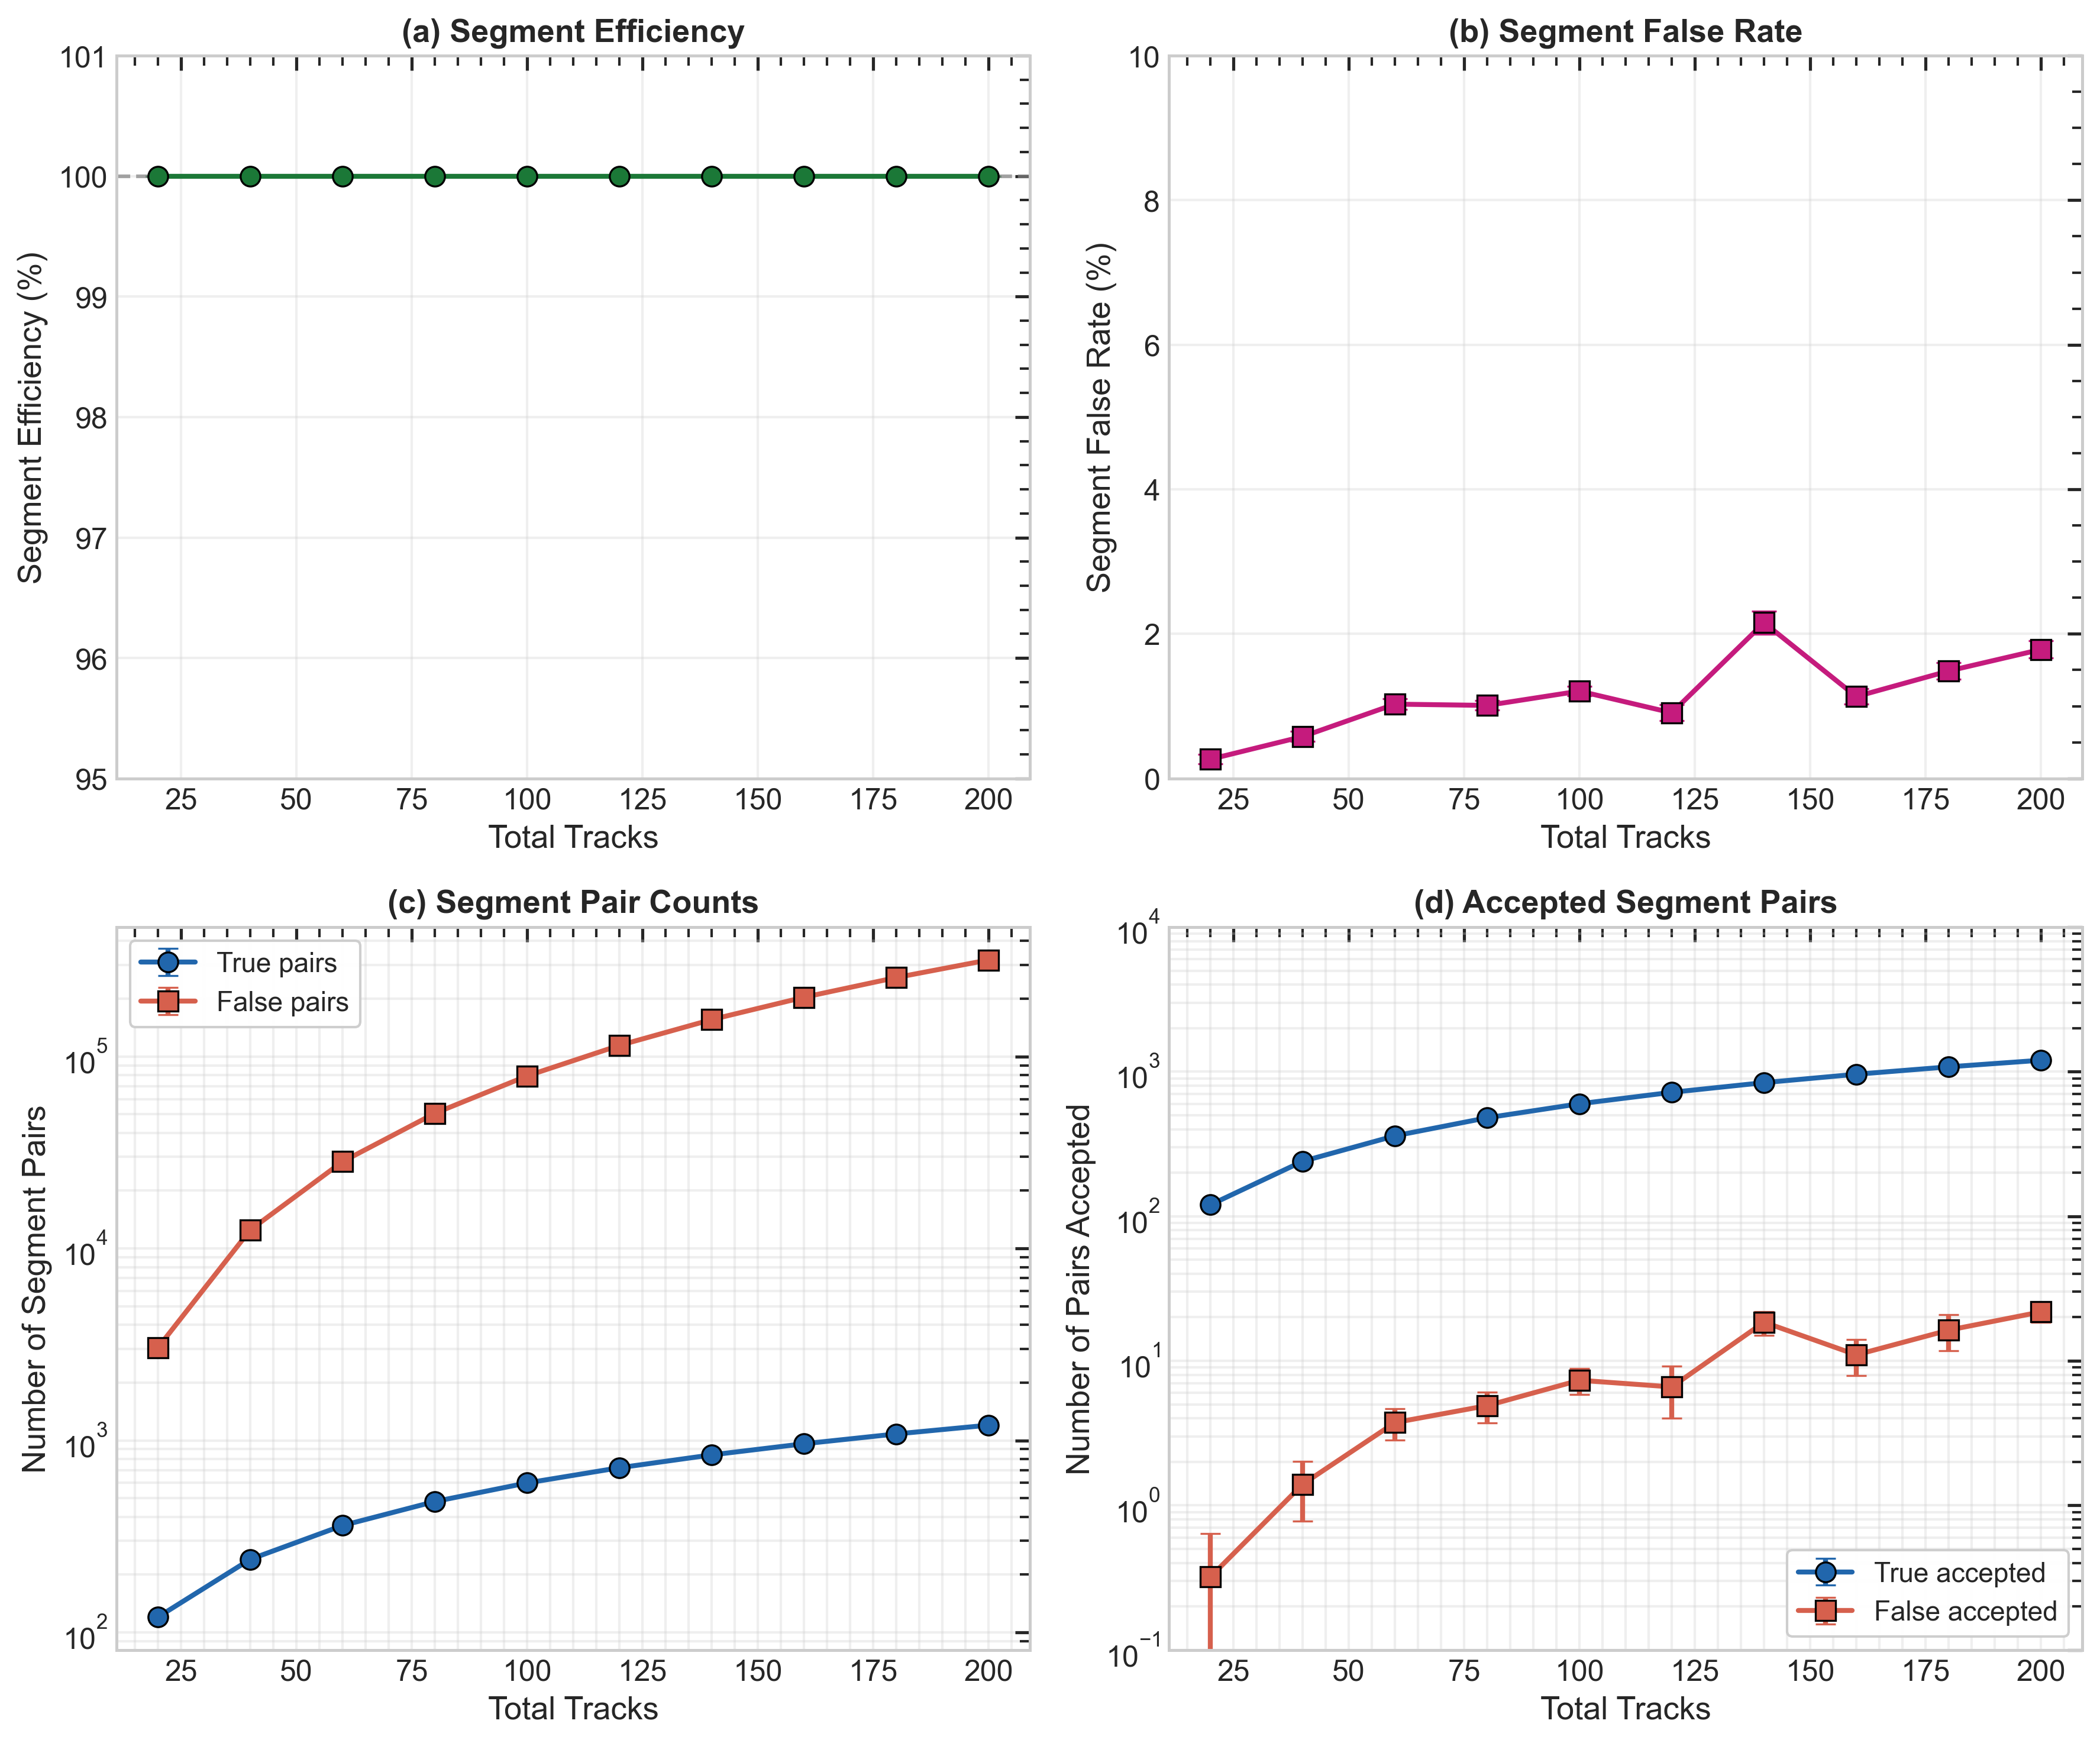
\includegraphics[width=0.85\textwidth]{segment_efficiency.png}
\caption{Segment-level performance of the Hamiltonian approach as a
function of total tracks (20--200). (a) Segment efficiency stays above
99.5\% across all densities. (b) False positive rate remains below 2\%
even at 200 tracks. (c) True and false segment pair counts on a log
scale. (d) Number of accepted true and false pairs after thresholding.
Error bars show standard deviation over 100 repeats.}
\label{fig:segment}
\end{figure}

\textbf{Panel (a) --- Segment Efficiency.} This measures what fraction of
true segment pairs the algorithm correctly identifies. It stays above
99.5\% from 20 tracks all the way up to 200 tracks. The Hamiltonian
approach is not missing real connections, even as the event becomes
denser.

\textbf{Panel (b) --- Segment False Rate.} This measures what fraction of
accepted segment pairs are actually fake. It stays below 1\% for most
configurations and only rises to about 2\% at the densest events (200
tracks). The slight increase is expected: as more particles are packed in,
the chance that two unrelated segments happen to be nearly collinear goes
up.

\textbf{Panel (c) --- Pair Counts.} The number of true pairs grows
roughly linearly with particle count (each new particle adds a fixed
number of segment pairs), while the number of false pairs grows
quadratically (all possible combinations between unrelated hits). By 200
tracks, false pairs outnumber true ones by about 10:1, but the threshold
still separates them cleanly.

\textbf{Panel (d) --- Accepted Pairs.} After applying the angular
threshold $\epsilon$, the number of accepted true pairs closely tracks the
total number of true pairs (consistent with panel (a)'s $>$99.5\%
efficiency). The number of accepted false pairs stays 1--2 orders of
magnitude below, confirming that the Hamiltonian's angular cut is
effective.

The takeaway is that the classical Hamiltonian reconstruction---the same
linear system $A\vec{S}=\vec{b}$ that the quantum algorithm solves---works
well even under realistic conditions and scales to high particle
densities. This validates the problem formulation itself, independent of
whether it is solved classically or quantumly.

% ======================================================================
\section{Circuit Complexity Scaling}

The example notebook reports gate counts for a single problem size (64
particles, 5 layers). The \texttt{plotting\_complexity.ipynb} notebook
analyses how circuit complexity scales as the problem size $N$ grows from
2 to 1024 particles. The data is pre-computed in
\texttt{data/circuit\_depth.json} (gate counts after transpilation for IBM
Torino hardware) and \texttt{data/success\_counts.json} (measurement
success rates from 100 million shots per run, 5 runs per configuration).

Figure~\ref{fig:complexity} shows the results.

\begin{figure}[H]
\centering
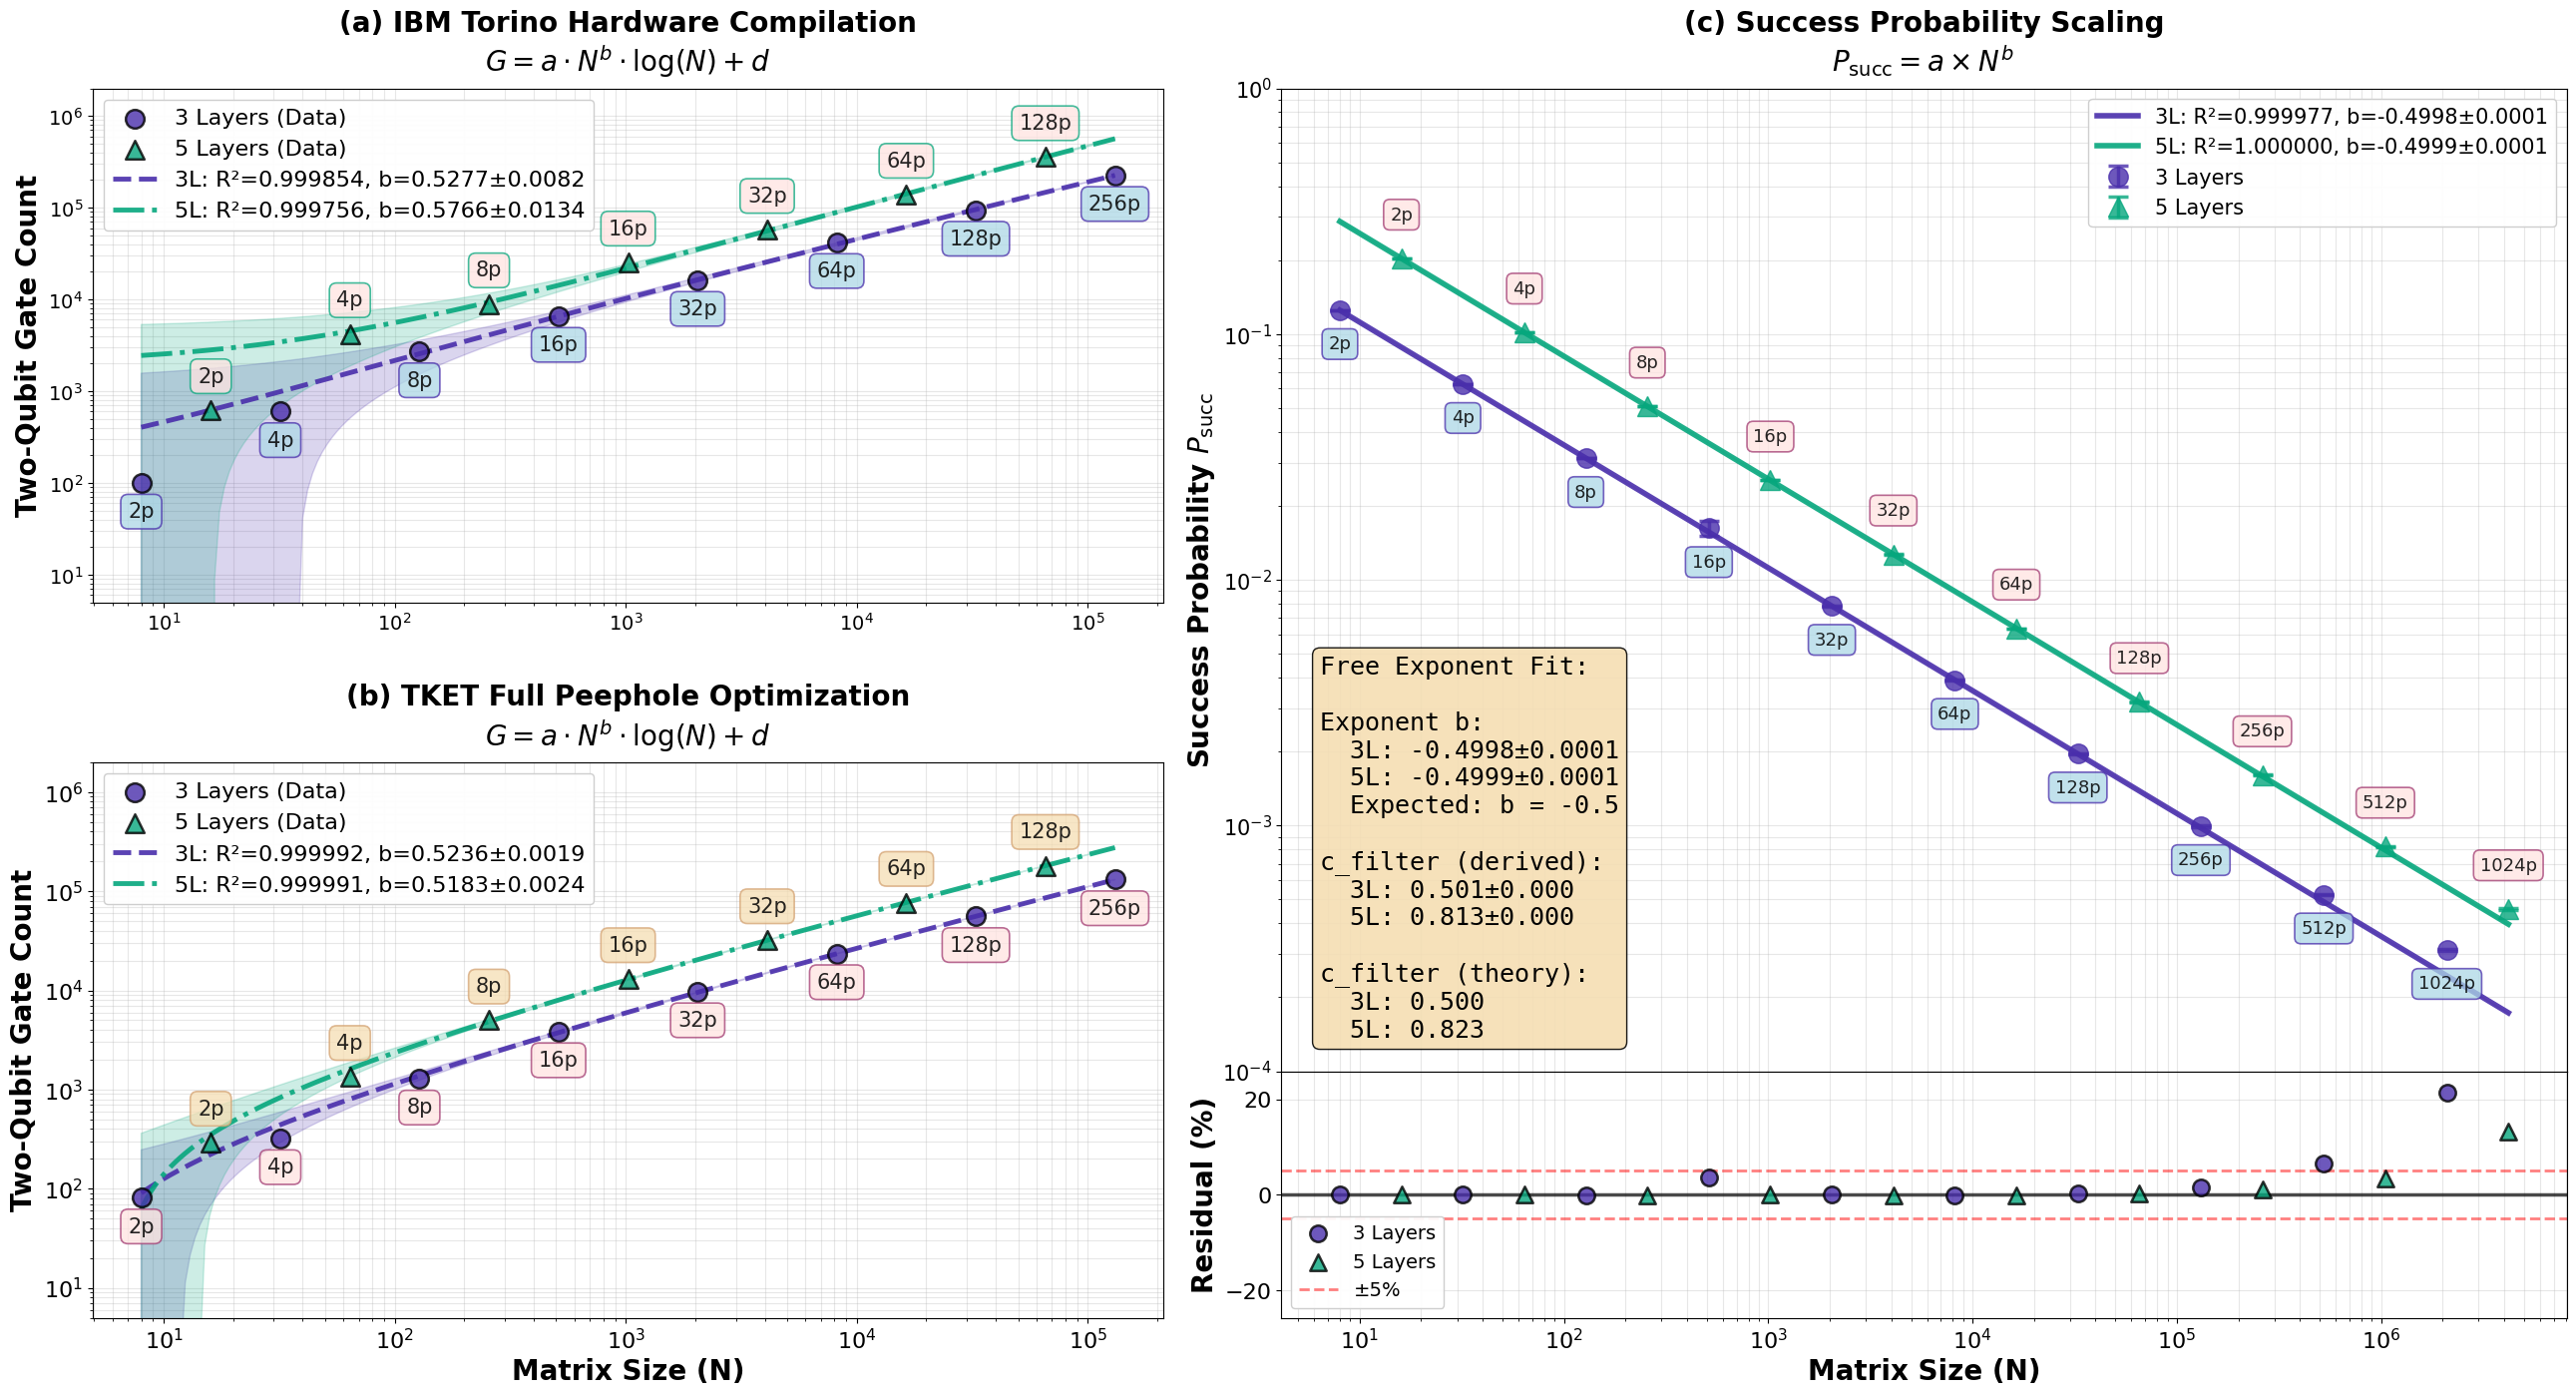
\includegraphics[width=\textwidth]{complexity_scaling.png}
\caption{Circuit complexity and success probability scaling. (a) Two-qubit
gate count after IBM Torino hardware transpilation, fitted as
$G = a \cdot N^b \cdot \log(N) + d$. (b) Same after TKET optimisation.
(c) Success probability $P_{\text{success}} = a \times N^b$ with
$b \approx -0.5$, matching the theoretical $1/\sqrt{N}$ prediction.
Bottom: fit residuals.}
\label{fig:complexity}
\end{figure}

\textbf{Panel (a) --- Qiskit / IBM Torino Compilation.} The two-qubit
gate count after transpilation for IBM Torino hardware is plotted against
matrix size $N$ on a log-log scale, for both 3-layer and 5-layer
problems. The fitted model is:
\begin{equation}
    G = a \cdot N^b \cdot \log(N) + d
\end{equation}
with the exponent $b \approx 0.53$ and $R^2 > 0.999$. The sub-linear
growth (exponent $< 1$) is significant: doubling the number of particles
less than doubles the gate count. For the largest problem tested (1024
particles, 5 layers), the circuit has roughly $4 \times 10^5$ two-qubit
gates after hardware compilation.

\textbf{Panel (b) --- TKET Optimisation.} The same data after TKET's
\texttt{FullPeepholeOptimise} pass. The scaling exponent is similar
($b \approx 0.52$), with a modest reduction in absolute gate counts. TKET
is most effective at reducing single-qubit gates rather than two-qubit
ones, which is why the improvement appears small on this plot (which
shows two-qubit gates only).

\textbf{Panel (c) --- Success Probability.} The probability of the
ancilla qubit measuring $\ket{1}$ (i.e.\ the post-selection success rate)
is fitted as $P_{\text{success}} = a \times N^b$, giving $b \approx
-0.5$. This matches the theoretical prediction that success probability
scales as $1/\sqrt{N}$. For 1024 particles the success rate is a few
percent, meaning that out of 100 million shots, several million give valid
post-selected results---more than enough for accurate solution extraction.

The residual panel at the bottom shows deviations from the fit are within
$\pm 5\%$, confirming the power-law model is a good description of the
scaling.

\subsection{What the Scaling Means}

The combination of sub-linear gate growth and $1/\sqrt{N}$ success
probability means the algorithm remains practical at larger scales:

\begin{center}
\begin{tabular}{lrrrr}
\toprule
\textbf{Particles} & \textbf{Segments ($N$)} & \textbf{Qubits} & \textbf{2Q Gates (Torino)} & \textbf{$P_{\text{success}}$} \\
\midrule
2   & 16       & 6  & $\sim$350          & $\sim$25\% \\
8   & 256      & 10 & $\sim$3{,}000      & $\sim$12\% \\
64  & 16{,}384 & 16 & $\sim$35{,}000     & $\sim$3\% \\
256 & 262{,}144 & 20 & $\sim$180{,}000   & $\sim$1.5\% \\
\bottomrule
\end{tabular}
\end{center}

Even at 256 particles, the circuit has under 200{,}000 two-qubit gates
and a success rate above 1\%. For context, current IBM quantum processors
support circuits with up to a few thousand two-qubit gates before noise
dominates, so the 2--8 particle range is the most realistic for
near-term hardware. The larger configurations would require error
correction.

% ======================================================================
\section{Fidelity and Noise Analysis}

The example notebook uses a perfect noiseless simulator. In practice,
quantum hardware introduces errors through imperfect gates, decoherence,
and crosstalk. The \texttt{plot\_fidelity\_results.ipynb} notebook
analyses how the OneBQF algorithm performs under realistic noise
conditions, using data from \texttt{data/fidelity\_results.json}.

The noise data was generated by running the OneBQF circuit through:
\begin{itemize}
    \item \textbf{IBM backends}: noise models extracted from real IBM
          quantum processors (Fez, Pittsburgh, Torino). These capture the
          actual gate error rates, readout errors, and crosstalk of
          specific hardware.
    \item \textbf{Quantinuum H2-Emulator}: a noise model based on
          Quantinuum's trapped-ion H2 processor, which generally has
          lower error rates than superconducting hardware.
\end{itemize}

Each configuration was run 10 times per backend. The noiseless simulator
serves as the baseline for comparison. Two metrics are computed:

\textbf{Hellinger Fidelity.} This measures how similar the noisy output
probability distribution is to the noiseless baseline, with 1.0 meaning
identical and 0.0 meaning completely different:
\begin{equation}
    F_H(P, Q) = \left(\sum_i \sqrt{p_i \cdot q_i}\right)^2
\end{equation}

\textbf{Signal Separation Index (SSI).} This measures how distinguishable
true track segments are from noise segments in the output:
\begin{equation}
    \text{SSI} = \frac{\langle p_{\text{track}} \rangle}{\langle p_{\text{noise}} \rangle}
\end{equation}
An SSI of 1.0 means tracks and noise are indistinguishable; higher is
better.

Bootstrap resampling (1000 samples) provides error bars for both metrics.

Figure~\ref{fig:fidelity} shows the results.

\begin{figure}[H]
\centering
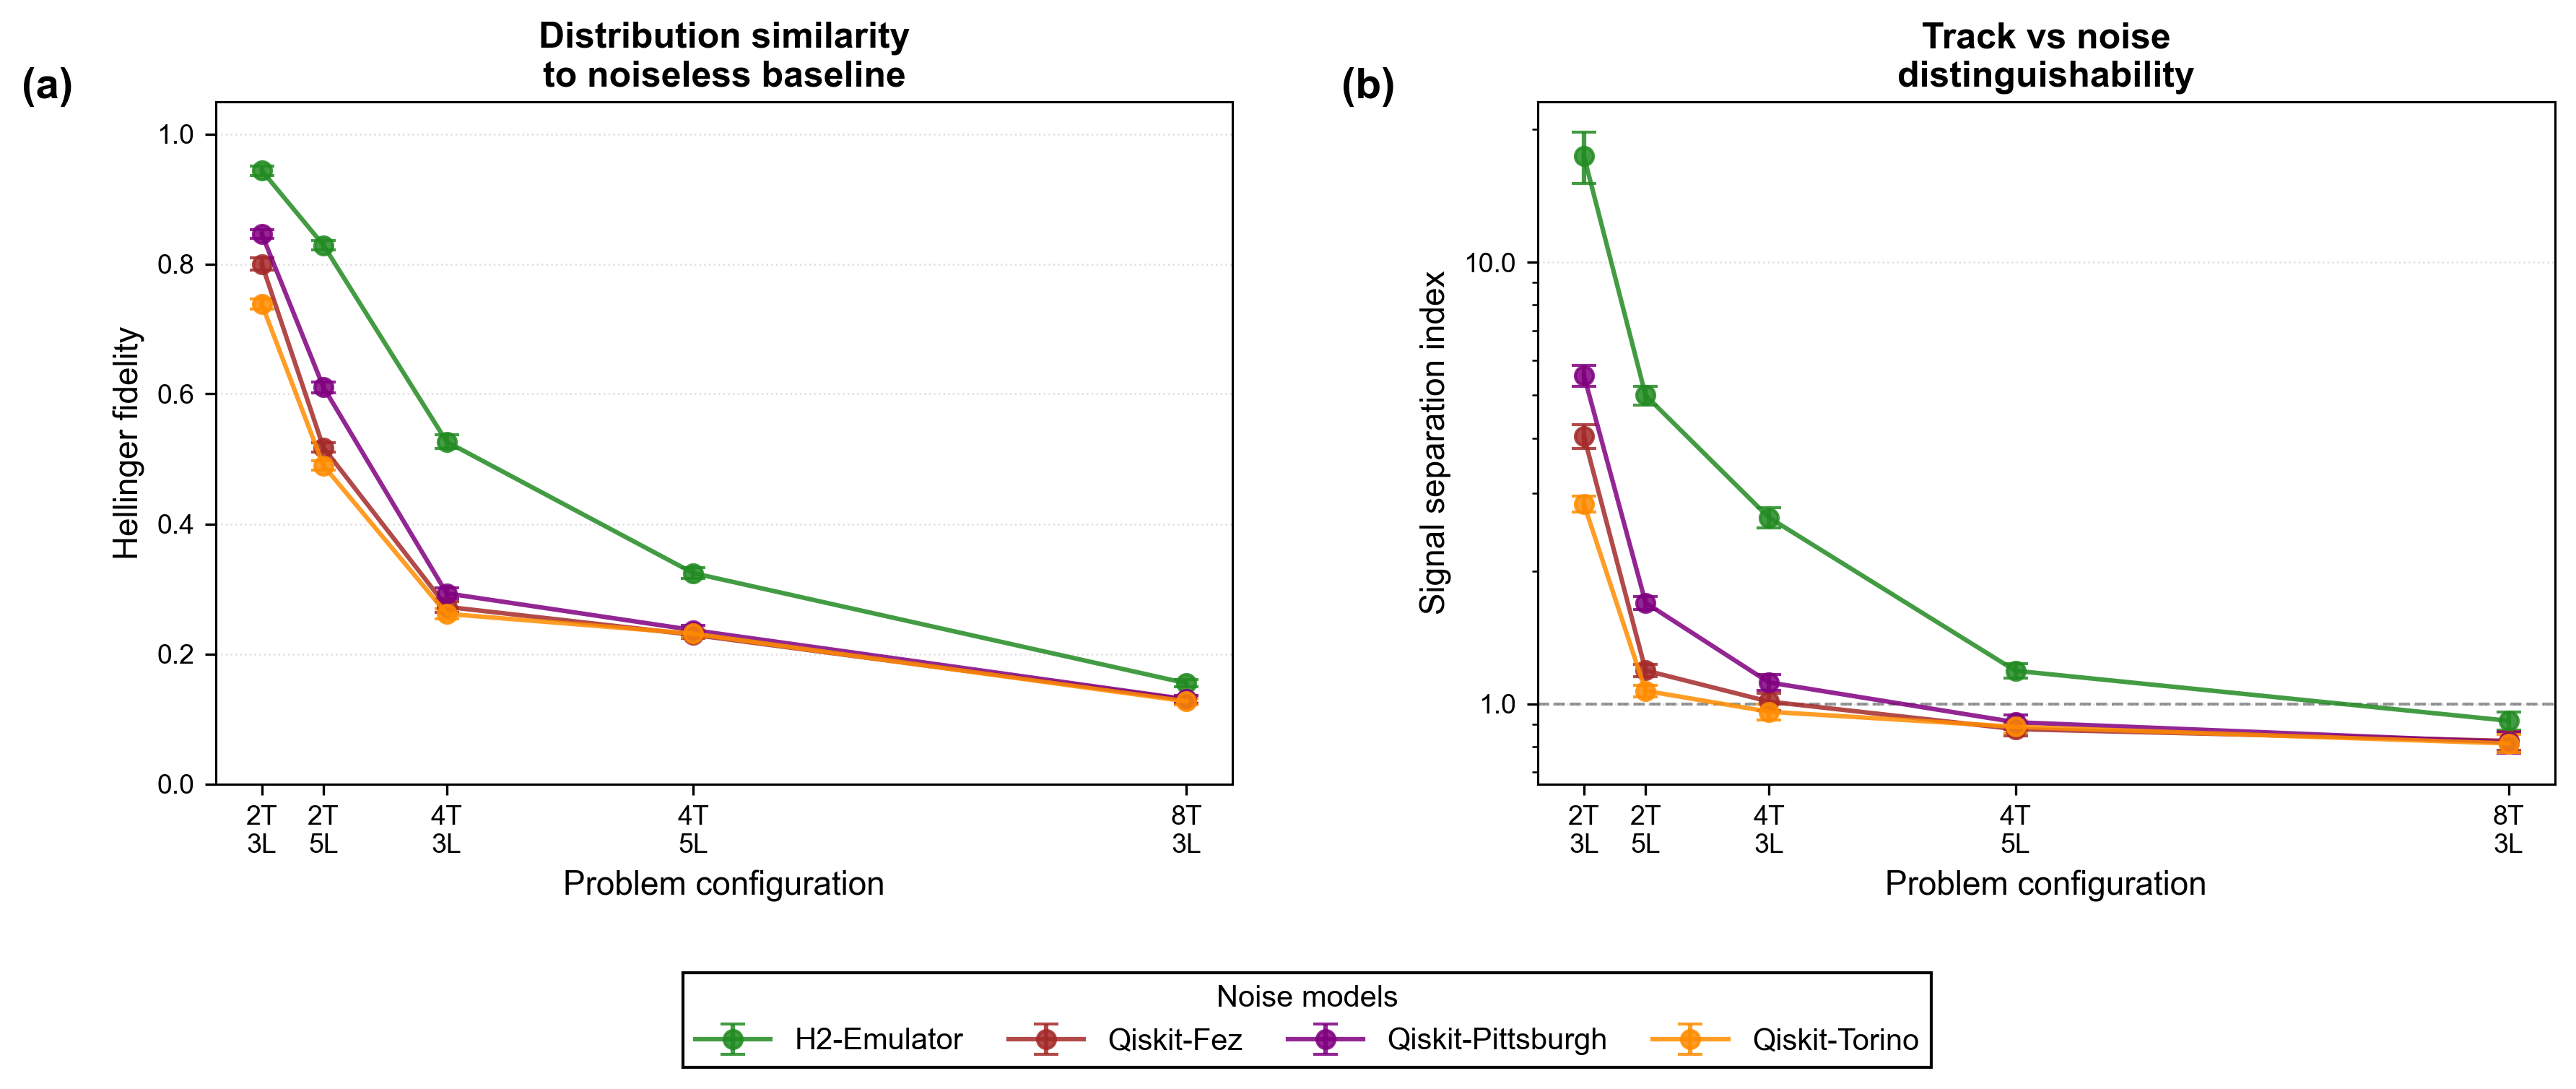
\includegraphics[width=\textwidth]{fidelity_noise.png}
\caption{Performance under noise. (a) Hellinger fidelity (similarity to
noiseless baseline) vs problem configuration. (b) Signal Separation Index
(track vs noise distinguishability). Problem configurations are labelled
as (particles)T\,(layers)L: ``2T 3L'' = 2 tracks, 3 layers. Four noise
models are compared: Quantinuum H2-Emulator (green), and IBM Qiskit
noise models for Fez (red), Pittsburgh (purple), and Torino (orange).}
\label{fig:fidelity}
\end{figure}

\textbf{Panel (a) --- Hellinger Fidelity.} For the smallest problems (2
tracks, 3 layers), the Quantinuum H2-Emulator achieves fidelity $\sim$0.9
and the IBM backends range from 0.6 to 0.85. As the problem size
increases, fidelity drops across all backends, reaching roughly 0.2 for 8
tracks with 3 layers. This is expected: larger circuits accumulate more
gate errors.

The Quantinuum emulator consistently outperforms the IBM noise models.
This reflects the generally lower gate error rates of trapped-ion systems
compared to superconducting qubits, particularly for two-qubit gates.

\textbf{Panel (b) --- Signal Separation Index.} For 2 tracks / 3 layers,
the H2-Emulator achieves an SSI above 10, meaning true track segments
are about 10 times more probable than noise segments in the output
distribution---even with hardware noise. The IBM backends achieve SSI
values of 2--5 for the same problem.

As problem size grows, all backends converge toward SSI $\approx$ 1.0,
meaning the noise eventually overwhelms the signal. The crossover point
where SSI drops below useful levels ($\sim$2) occurs around 4 tracks for
IBM backends and around 4--8 tracks for the Quantinuum emulator.

\subsection{Implications for Hardware}

The fidelity results show that the 1-Bit Quantum Filter can produce
meaningful results on current quantum hardware, but only for small problem
sizes (2--4 particles). At this scale, the circuit is shallow enough that
noise does not destroy the signal. For larger problems, error mitigation
or error correction would be needed.

The Quantinuum trapped-ion platform performs noticeably better, which
aligns with its lower two-qubit gate error rates ($\sim$0.1--0.3\%
compared to $\sim$0.5--1\% for IBM superconducting devices). Since the
OneBQF circuit's bottleneck is the number of CX/two-qubit gates (321 for
64 particles), platforms with lower two-qubit error rates will have a
significant advantage.

% ======================================================================
\section{Summary}

\subsection{The Example Notebook}

The notebook demonstrates a complete end-to-end pipeline:

\begin{enumerate}
    \item A simulated VELO detector with 5 layers generates 64 particle
          tracks, producing 16,384 candidate segments.
    \item A Hamiltonian is constructed that encodes track-finding as a
          linear system $A\vec{S} = \vec{b}$.
    \item The 1-Bit Quantum Filter solves this system using a 7-qubit
          quantum circuit with depth 507.
    \item The quantum solution perfectly matches the classical conjugate
          gradient solution: all 256 true segments are correctly
          identified with zero mismatches.
    \item The quantum solution has the additional property that inactive
          segments are fully suppressed to zero, making thresholding
          unnecessary.
\end{enumerate}

\subsection{The Scaling and Noise Studies}

Beyond the notebook, the paper's pre-computed data reveals how the
algorithm behaves at scale and under realistic conditions:

\begin{enumerate}
    \item \textbf{Segment efficiency} (Figure~\ref{fig:segment}): The
          Hamiltonian reconstruction correctly identifies $>$99.5\% of
          true segment pairs with $<$2\% false positives, even at 200
          particles with realistic noise and scattering.

    \item \textbf{Circuit scaling} (Figure~\ref{fig:complexity}): Gate
          counts grow sub-linearly ($\sim N^{0.53}$) and success
          probability follows $1/\sqrt{N}$, both matching theoretical
          predictions with $R^2 > 0.999$.

    \item \textbf{Hardware noise} (Figure~\ref{fig:fidelity}): The
          algorithm produces meaningful results on noisy hardware for
          2--4 particle problems. The Quantinuum H2-Emulator
          significantly outperforms IBM superconducting backends, with
          Hellinger fidelity near 0.9 and SSI $>$ 10 for the smallest
          problems.
\end{enumerate}

\subsection{Overall}

The 1-Bit Quantum Filter correctly solves the track reconstruction
problem on a noiseless simulator for up to 64 particles, with circuit
complexity roughly 1000 times smaller than naive HHL. On noisy hardware,
it produces usable results for 2--4 particles. Scaling to HL-LHC
conditions (1500 particles) would require $\sim$26 qubits and
error-corrected hardware, but the sub-linear gate scaling and efficient
post-selection make this a credible long-term path.

\end{document}
